\documentclass[tikz]{standalone}
\begin{document}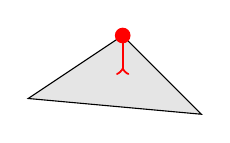
\begin{tikzpicture}
\coordinate (x) at (0,0);
\coordinate (y) at (-1.2,-.8);
\coordinate (z) at (1,-1);
\filldraw[draw=black,fill=gray!20] (x) -- (y) -- (z) -- cycle;

\draw[thick,red,-<] (x) -- +(0,-.5);
\node[fill,circle,red,inner sep=2pt] at (x) {};

\end{tikzpicture}\end{document}
